\section{Aggiungere il supporto a \texttt{make} in alcuni editor di testo}
\label{sec:editor}

Può essere utile poter richiamare \texttt{make} direttamente dal proprio editor
di testo preferito.  In generale consiglio di aggiungere il comando
\texttt{make} all'elenco dei comandi di composizione dell'editor, in modo da
poter eseguire la regola predefinita del \texttt{Makefile}.  Di seguito sono
riportate le istruzioni per aggiungere \texttt{make} all'elenco dei programmi di
composizione di alcuni dei più diffusi editor di testo specifici per \LaTeX{}.
Affinché tutti gli editor di testo possano effettuare correttamente l'analisi
dell'output di \texttt{make} è necessario compilare in modalità
\texttt{nonstopmode}.  Questo può essere fatto aggiungendo nel \texttt{Makefile}
ai comandi \texttt{latex} o \texttt{pdflatex} (o l'eventuale altro compilatore
usato) l'opzione \texttt{-interaction=nonstopmode}
\begin{lstlisting}
$(PRINCIPALE_DVI): $(TUTTI_LATEX) immagini-eps
	latex -interaction=nonstopmode $(PRINCIPALE)
	bibtex $(PRINCIPALE)
	makeindex $(PRINCIPALE)
	latex -interaction=nonstopmode $(PRINCIPALE)
	latex -interaction=nonstopmode $(PRINCIPALE)

$(PRINCIPALE_PDF): $(TUTTI_LATEX) $(IMMAGINI_PDF)
	pdflatex -interaction=nonstopmode $(PRINCIPALE)
	bibtex $(PRINCIPALE)
	makeindex $(PRINCIPALE)
	pdflatex -interaction=nonstopmode $(PRINCIPALE)
	pdflatex -interaction=nonstopmode $(PRINCIPALE)
\end{lstlisting}

\subsection{Emacs}
\label{sec:emacs}

Aggiungere al proprio file di inizializzazione \texttt{.emacs} il seguente codice
\begin{lstlisting}[language=lisp,morekeywords={eval-after-load}]
(eval-after-load "tex"
  (add-to-list 'TeX-command-list
	       '("Make" "make" TeX-run-TeX nil t)))
\end{lstlisting}
È necessario utilizzare il pacchetto AUC\TeX{}.
Con questa modifica sarà possibile eseguire \texttt{make} con
\texttt{C-c C-c Make RET}.

\subsection{Texmaker}
\label{sec:texmaker}

\begin{figure}
  \centering
  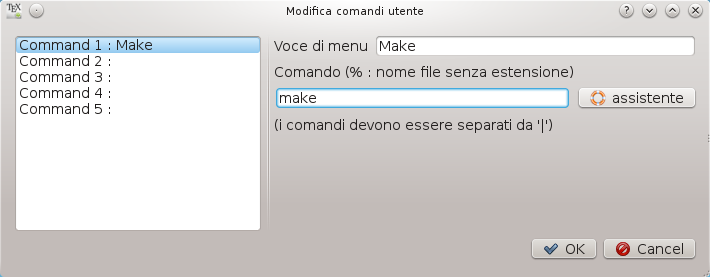
\includegraphics[width=0.8\textwidth]{figure/texmaker}
  \caption{Finestra di configurazione di Texmaker.}
  \label{fig:texmaker}
\end{figure}
Seguendo il menu
\menu{Utente > Comandi personalizzati > Modifica comandi utente} si aprirà una
finestra come quella riportata nella figura~\ref{fig:texmaker} e si deve
scrivere ``Make'' nel campo ``Voce di menu'' e ``make'' nel campo ``Comando''.
In questo modo \texttt{make} sarà eseguibile dall'elenco dei comandi
personalizzati.

\subsection{TeXstudio}
\label{sec:texstudio}

\begin{figure}
  \centering
  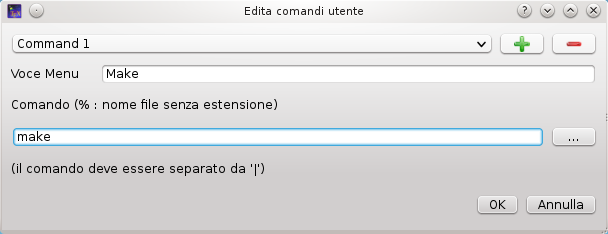
\includegraphics[width=0.8\textwidth]{figure/texstudio}
  \caption{Finestra di configurazione di TeXstudio.}
  \label{fig:texstudio}
\end{figure}
TeXstudio è un fork di Texmaker e la procedura è simile a quella descritta qui
sopra.  Dal menu \menu{Utente > Comandi utente > Edit comandi utente} si aprirà
una finestra come quella riportata nella figura~\ref{fig:texstudio} e nel campo
``Voce menu'' si scriverà ``Make'', nel campo ``Comando'' si scriverà ``make''.
Dopo di ciò sarà possibile eseguire \texttt{make} dall'elenco dei comandi
utente.

\subsection{Texworks}
\label{sec:texworks}

\begin{figure}
  \centering
  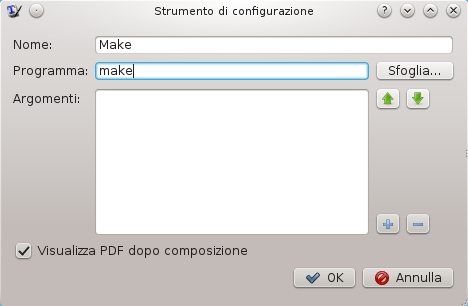
\includegraphics[width=0.8\textwidth]{figure/texworks}
  \caption{Finestra di configurazione di Texworks.}
  \label{fig:texworks}
\end{figure}
Andare nel menu \menu{Modifica > Preferenze} e nella scheda ``Composizione''
della finestra che si aprirà fare clic sul pulsante \keys{{+}} vicino all'elenco
degli strumenti di composizione.  Nella finestra che si aprirà, come quella
riportata nella figura~\ref{fig:texworks}, scrivere ``Make'' nel campo ``Nome''
e ``make'' nel campo ``Programma''.  Dopo di ciò \texttt{make} sarà disponibile
nell'elenco dei programmi di composizione di questo editor di testo.

%%% Local Variables:
%%% mode: latex
%%% TeX-master: "../make"
%%% End:
